%%%%%%%%%%%%%%%%%%%%%%%%%%%%%%%%%%%%%%%%%
%
% Reproducible Research Workshop Slides
% Module 03
% Perry Williams
% 09/12/2020
%
%%%%%%%%%%%%%%%%%%%%%%%%%%%%%%%%%%%%%%%%%

% ---------------------------------------------------------
%	PACKAGES AND THEMES
% ---------------------------------------------------------

\documentclass{beamer}\usepackage[]{graphicx}\usepackage[]{color}
% maxwidth is the original width if it is less than linewidth
% otherwise use linewidth (to make sure the graphics do not exceed the margin)
\makeatletter
\def\maxwidth{ %
  \ifdim\Gin@nat@width>\linewidth
    \linewidth
  \else
    \Gin@nat@width
  \fi
}
\makeatother

\definecolor{fgcolor}{rgb}{0.345, 0.345, 0.345}
\newcommand{\hlnum}[1]{\textcolor[rgb]{0.686,0.059,0.569}{#1}}%
\newcommand{\hlstr}[1]{\textcolor[rgb]{0.192,0.494,0.8}{#1}}%
\newcommand{\hlcom}[1]{\textcolor[rgb]{0.678,0.584,0.686}{\textit{#1}}}%
\newcommand{\hlopt}[1]{\textcolor[rgb]{0,0,0}{#1}}%
\newcommand{\hlstd}[1]{\textcolor[rgb]{0.345,0.345,0.345}{#1}}%
\newcommand{\hlkwa}[1]{\textcolor[rgb]{0.161,0.373,0.58}{\textbf{#1}}}%
\newcommand{\hlkwb}[1]{\textcolor[rgb]{0.69,0.353,0.396}{#1}}%
\newcommand{\hlkwc}[1]{\textcolor[rgb]{0.333,0.667,0.333}{#1}}%
\newcommand{\hlkwd}[1]{\textcolor[rgb]{0.737,0.353,0.396}{\textbf{#1}}}%
\let\hlipl\hlkwb

\usepackage{framed}
\makeatletter
\newenvironment{kframe}{%
 \def\at@end@of@kframe{}%
 \ifinner\ifhmode%
  \def\at@end@of@kframe{\end{minipage}}%
  \begin{minipage}{\columnwidth}%
 \fi\fi%
 \def\FrameCommand##1{\hskip\@totalleftmargin \hskip-\fboxsep
 \colorbox{shadecolor}{##1}\hskip-\fboxsep
     % There is no \\@totalrightmargin, so:
     \hskip-\linewidth \hskip-\@totalleftmargin \hskip\columnwidth}%
 \MakeFramed {\advance\hsize-\width
   \@totalleftmargin\z@ \linewidth\hsize
   \@setminipage}}%
 {\par\unskip\endMakeFramed%
 \at@end@of@kframe}
\makeatother

\definecolor{shadecolor}{rgb}{.97, .97, .97}
\definecolor{messagecolor}{rgb}{0, 0, 0}
\definecolor{warningcolor}{rgb}{1, 0, 1}
\definecolor{errorcolor}{rgb}{1, 0, 0}
\newenvironment{knitrout}{}{} % an empty environment to be redefined in TeX

\usepackage{alltt}

\usetheme{Madrid}
\usecolortheme{beaver}

\setbeamertemplate{navigation symbols}{}
\setbeamercolor{block title}{fg=black,bg=darkred}
\setbeamercolor{block body}{fg=black,bg=lightgray}


\usepackage{animate}
\usepackage{booktabs}
\usepackage{graphicx}
\usepackage{mathtools}
\usepackage{mathrsfs}
\usepackage{media9}
\usepackage{listings}
\usepackage{pgf}
\usepackage{stackengine}
\usepackage{textpos}
\usepackage{tikz}
\usepackage{xcolor}
\lstset{breaklines=true} % break long lines
\newcommand\Fontvi{\fontsize{14}{7.2}\selectfont}
\newcommand{\backupbegin}{
  \newcounter{finalframe}
  \setcounter{finalframe}{\value{framenumber}}
}
\newcommand{\backupend}{
  \setcounter{framenumber}{\value{finalframe}}
}
\renewcommand\useanchorwidth{T}
\def\theyearwidth{1.5pt}
\newlength\yrsfboxrule
\yrsfboxrule .4\fboxrule
\newcommand\yearwidth[1]{\def\theyearwidth{#1}\ignorespaces}
\newcommand\skipyears[2][white]{%
  \fboxrule\yrsfboxrule%
  \fboxsep=-\yrsfboxrule%
  \fcolorbox{gray}{#1}{\strut\hspace{#2}}%
  \ignorespaces%
}
\newcommand\showyear[2][black]{%
  \fboxsep=0pt%
  \stackon{%
    \colorbox{#1}{\strut\hspace{\theyearwidth}}
  }{\sffamily\small#2}%
  \ignorespaces%
}

\let\svthefootnote\thefootnote
\textheight 1in
\newcommand\blankfootnote[1]{%
  \let\thefootnote\relax\footnotetext{#1}%
  \let\thefootnote\svthefootnote%
}
\usetikzlibrary{fadings}
\tikzfading[name=fade out, inner color=transparent!0,
         outer color=transparent!100]

\graphicspath{{./Images/}}

% ---------------------------------------------------------
%	TITLE PAGE
% ---------------------------------------------------------

\title[Reproducible Research]{\normalsize GRAD 778: Reproducible Research}
\author[Perry Williams]{\footnotesize Perry J. Williams}
\vspace{1in}
\institute[]{
  Ecological Statistician \\
  Department of Natural Resources and Environmental Science\\
  University of Nevada, Reno}
\date[09/21/2019]{09/21/2019}
\IfFileExists{upquote.sty}{\usepackage{upquote}}{}
\begin{document}

\begin{frame}
\begin{textblock*}{4cm}(8cm,5.8cm) % {block width} (coords)
      \begin{tikzpicture} \path (0,0) rectangle
        (5,7); \node[scope fading=fade out,inner
        sep=0pt,outer sep=0pt,anchor=south east]
        at(5,5)
        {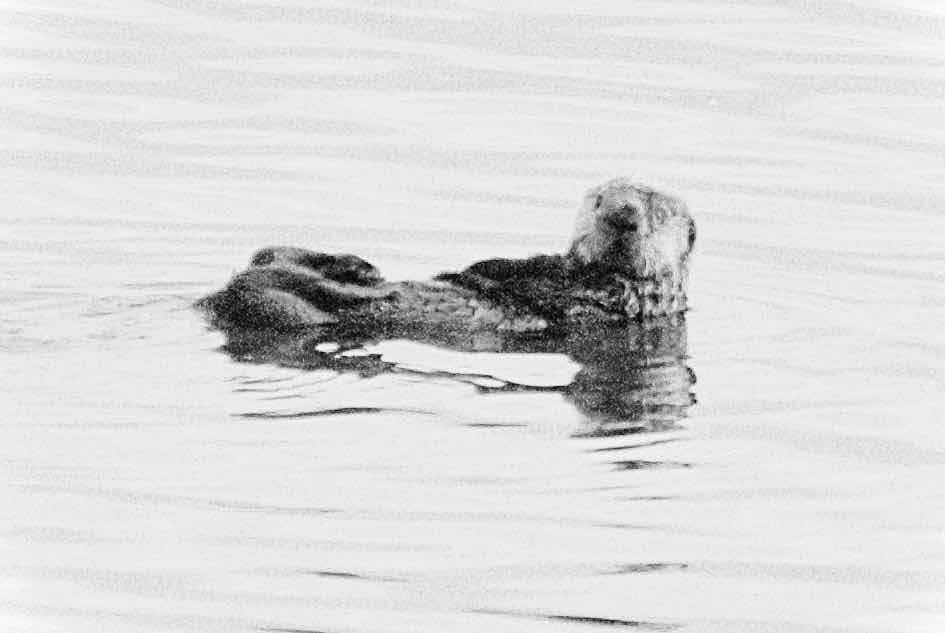
\includegraphics[width=5cm]{icon2}};
      \end{tikzpicture}
  \end{textblock*}
\begin{textblock*}{4cm}(-2cm,5.5cm) % {block width} (coords)
      \begin{tikzpicture} \path (0,0) rectangle
        (5,7); \node[scope fading=fade out,inner
        sep=0pt,outer sep=0pt,anchor=south east]
        at(5,5)
        {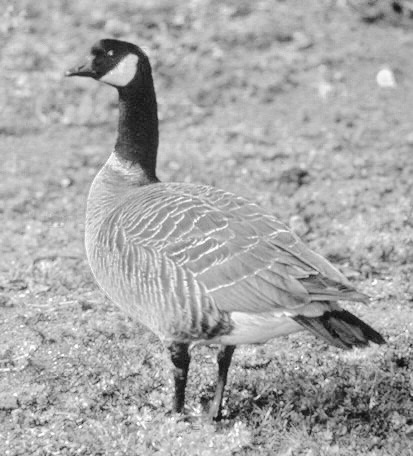
\includegraphics[width=3cm]{cago3}};
      \end{tikzpicture}
  \end{textblock*}
  \titlepage
\end{frame}

% -------------------------------------------------------
% PRESENTATION SLIDES
% -------------------------------------------------------

% ------------------------------------------------
\section{Using \LaTeX}
% ------------------------------------------------


\begin{frame}[noframenumbering]
  \begin{center}
      \textsc{\textrm{Using \LaTeX}}

   \end{center}
\end{frame}

\begin{frame}{Basic \LaTeX command syntax}
  \begin{itemize}
  \item Latex command begin with a backslash
  \item The arguments for Latex commands are written inside of curly braces
  \item Comments are made with a \% sign
  \end{itemize}
\end{frame}


\begin{frame}[fragile]
  \begin{lstlisting}
    \documentclass{article}


     \title{My First \LaTeX Document}
     \author{Jane Doe}
     \date{September 2019}

     \begin{document}
     \maketitle
     Hello world!
     \end{document}

\end{lstlisting}
\end{frame}

\begin{frame}
  \begin{center}
    
\includegraphics[width=.8\linewidth,keepaspectratio]{latex1}
  \end{center}
\end{frame}


\begin{frame}[fragile]
  \tiny
  \begin{lstlisting}
    \documentclass{article}

    \usepackage{lipsum}

    \title{My Second \LaTeX Document}
    \author{Jane Doe}
    \date{September 2019}

    \begin{document}
    \maketitle
    \section{Abstract}
    \lipsum[2-4]

    \section{Introduction}
    \lipsum[2-4]

    \section{Methods}
    \lipsum[2-4]

    \section{Results}
    \lipsum[2-4]

    \section{Discussion}
    \lipsum[2-4]

    \end{document}

\end{lstlisting}
\end{frame}

\begin{frame}
  \begin{columns}
    \begin{column}{0.5\textwidth}
      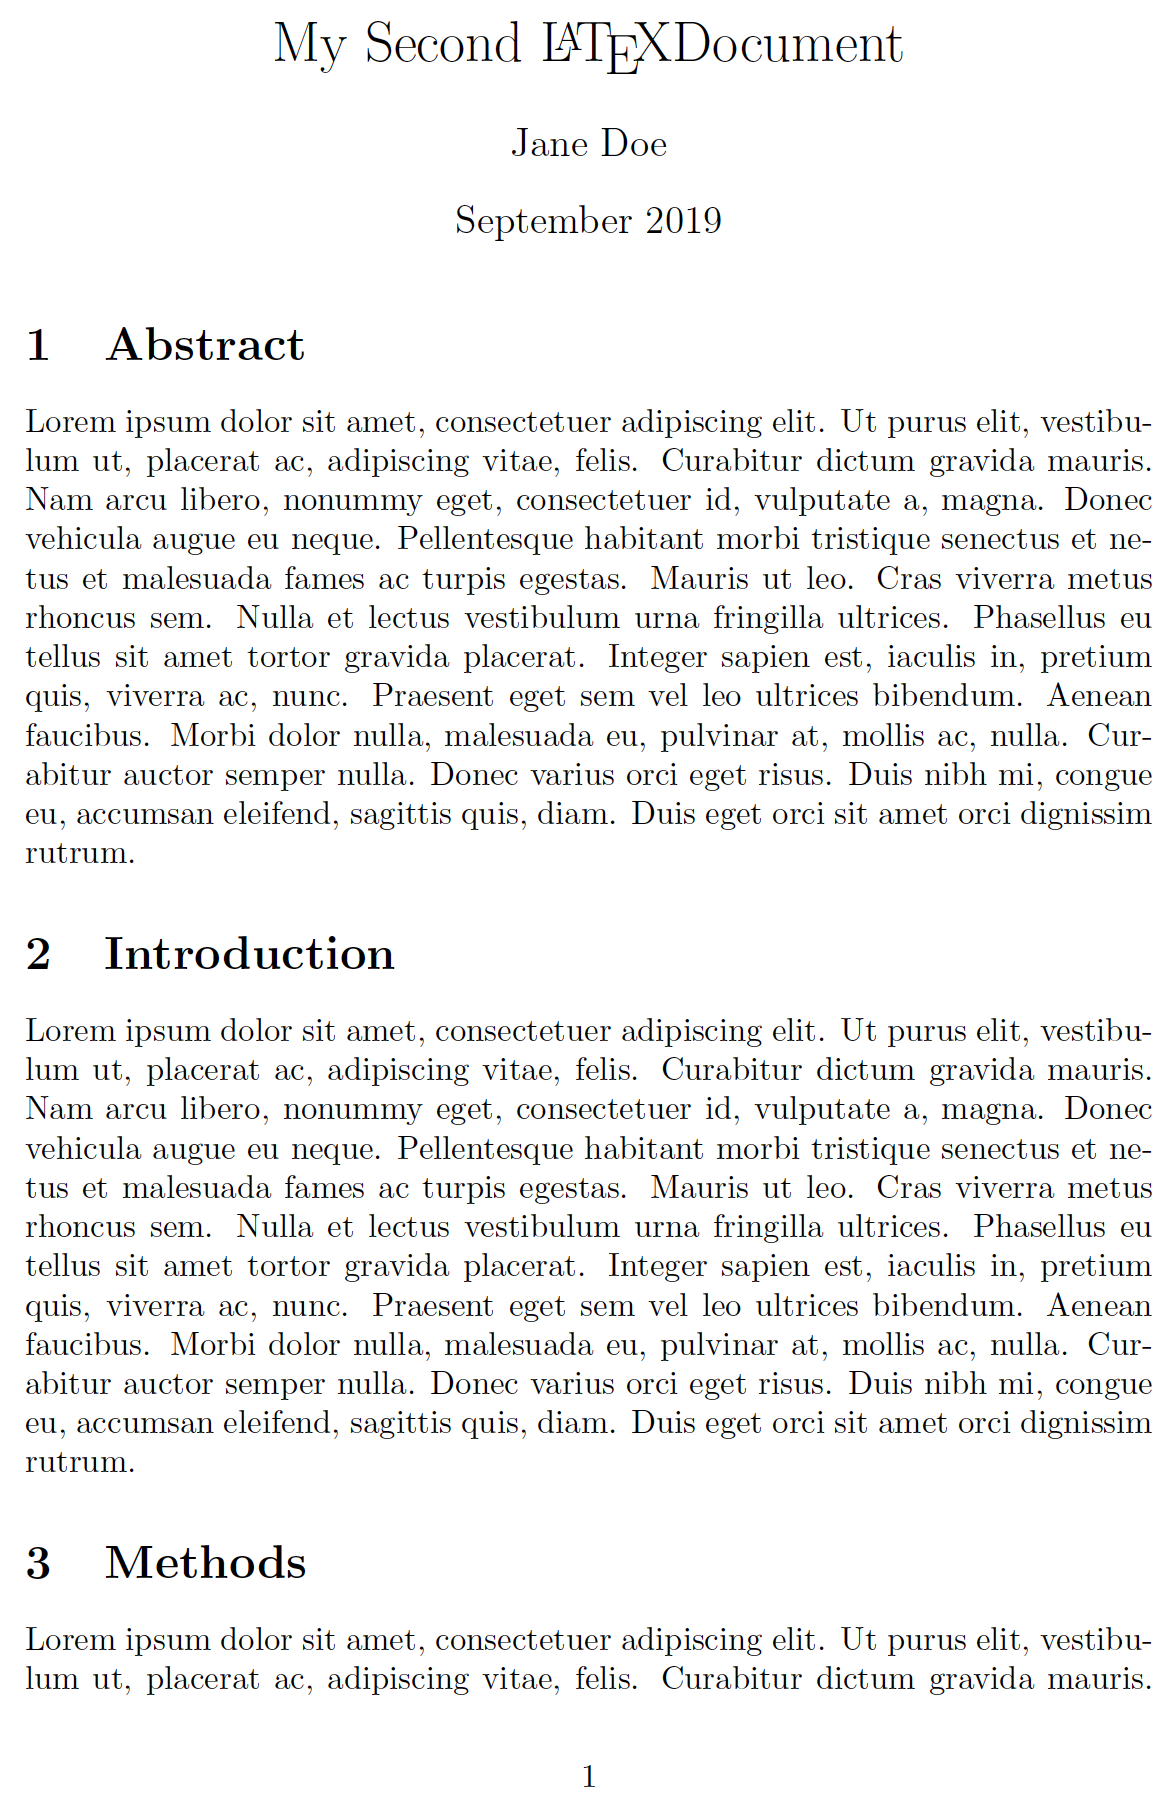
\includegraphics[width=.8\linewidth,keepaspectratio]{latex2a}
    \end{column}
    \begin{column}{0.5\textwidth}
      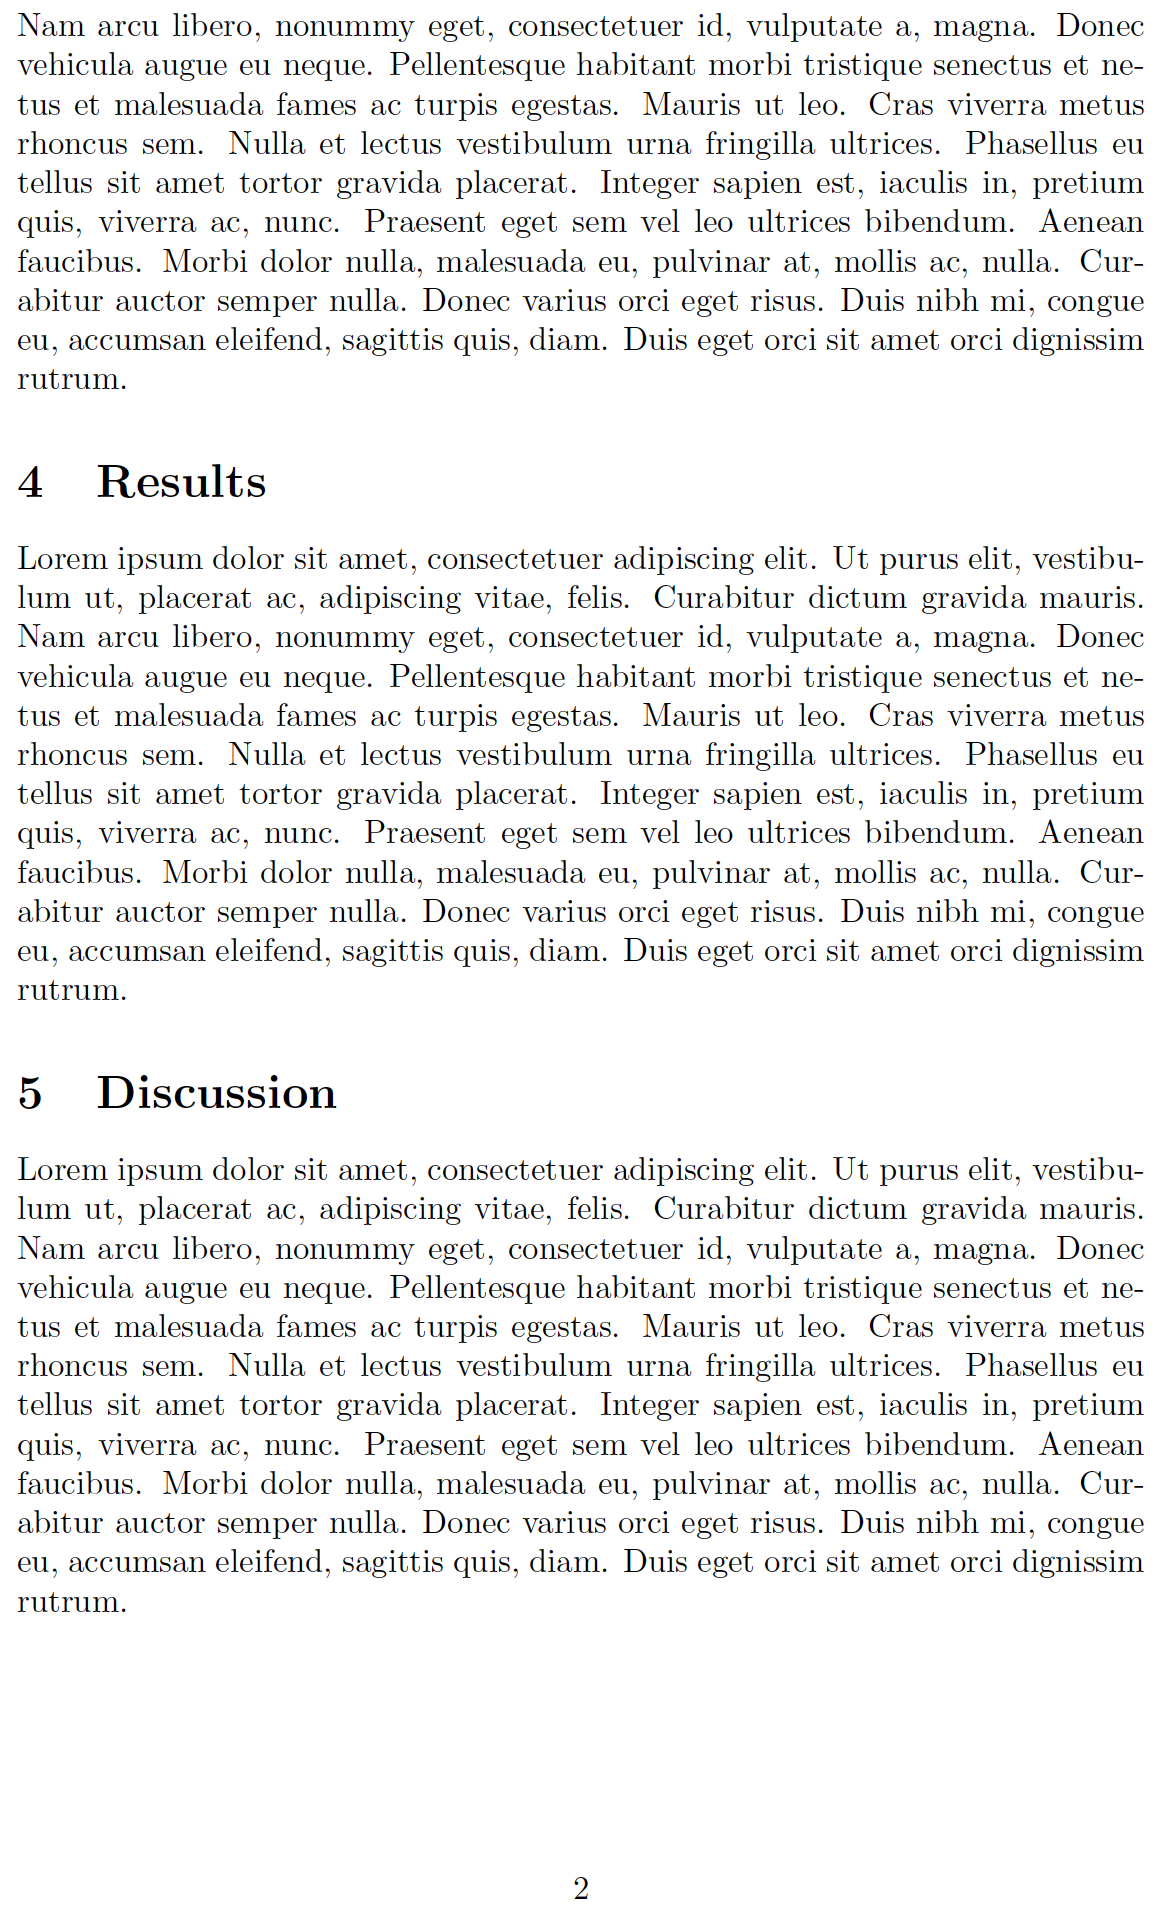
\includegraphics[width=.8\linewidth,keepaspectratio]{latex2b}
    \end{column}
  \end{columns}
\end{frame}

\begin{frame}{Exercise 1}
\footnotesize
\textbf{Using \LaTeX templates}
  \begin{itemize}
  \item Navigate to the folder: \texttt{/GRAD778\_04\_2020/Presentation/Module03\_LaTeX/LaTeXExercise/}
  \item Choose one of the templates from the journals Ecography, Journal of Animal Ecology (JAE), Journal of Wildlife Management (JWM), Proceedings of the National Academy of Science (PNAS), or Science.
  \item   Open the \texttt{.tex} file in the folder.
  \item Customize the template to include:
  \begin{itemize}
  \item Author names from a publication/project you are working on,
  \item Affiliations,
  \item Sections and sub-sections relevant for your work.
  \end{itemize}
  \item   Open the \texttt{.bib} file in the folder.
  \item Customize the .bib file to include:
  \begin{itemize}
  \item A reference from your field (go to Google Scholar, find an appropriate article, select the quotation marks below the article, and select "BibTeX" at the bottom of the pop-up window. Copy and past it into the .bib file)
  \end{itemize}
  \item Add the handle of the reference to the main .tex article using citep\{handle\} (with a backslash before citep).
\end{itemize}
\end{frame}

\end{document}


